
In this section, we the role of eye movements specific to action planning and execution. The action of picking up an object and dropping it to a shelf location requires precise attention on the object to be grasped and then a shift of gaze to the location of the place where the object will be dropped off. The change of proportion of fixations on the task-relevant objects of interest over time would reveal the average shift of gaze before and during the action execution. To do this, we employ seven regions-of-interest for each action of displacing an object. These regions-of-interest consist of the current target object (current\_TO) that is being displaced, the current target shelf (current\_TS) where the object is displaced finally, the previous target object (prev\_TO) and previous target shelf (prev\_TS) that were relevant in the previous action, the next target object (next\_TO) and next target shelf (next\_TS) that will be interacted with in the next action in the sequence, and finally all the other objects and shelves that were not relevant in the action sequence. We selected the 3s before the virtual hand touches the object (grasp onset) and 3s after and divided it into 0.25 second bins to calculate the proportion of fixations on all of the ROIs within each time bin. Hence, we can assess the dynamic changes in the proportion of fixations on the seven ROIs as the current action is planned and executed.

\begin{figure}[h]
    \centering
    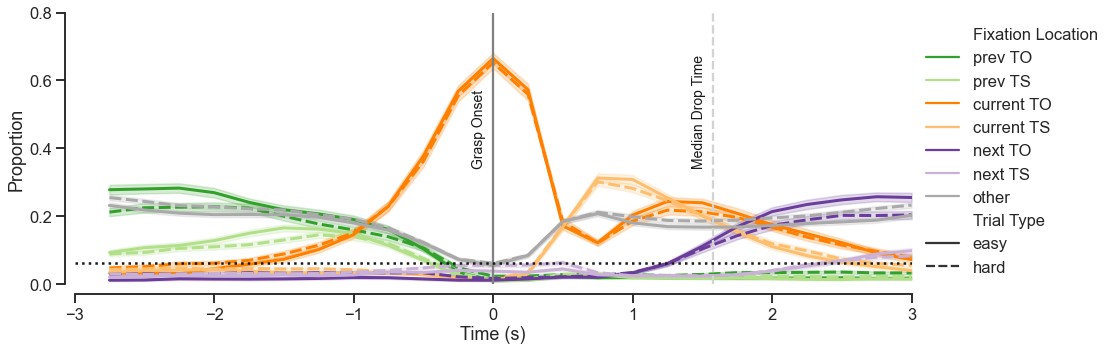
\includegraphics[width=0.9\linewidth]{source/figures/results/time_course_proportion_7ROI.png}
    \label{figure:timecourse_fixprop}\\
    % \subfloat[]{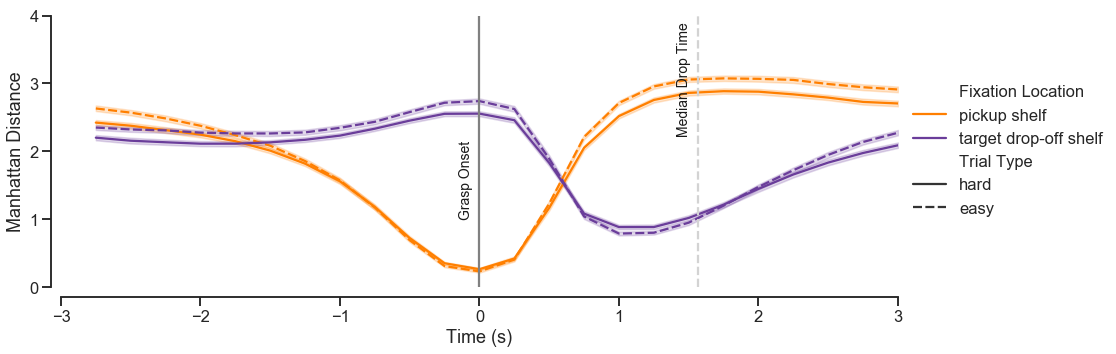
\includegraphics[width=0.7\linewidth]{source/figures/results/time_course_fix_distance.png}
    % \label{figure:timecourse_manhattan}}
    \caption[]{ Time course of proportion of fixations centered on the object displacement initiation (grasp onset) at time=0 and 3 seconds before and after on the seven regions of interest and for the two trial types (EASY and HARD). The black dotted horizontal line indicate the chance level (1/16)  of fixating on a target object. The shaded regions show 95\% confidence interval of the mean proportion of gaze at each time-bin across all trials within a trial type. These regions-of-interest consist of the current target object (current\_TO) that is being displaced, the current target shelf (current\_TS) where the object is displaced finally, the previous target object (prev\_TO) and previous target shelf (prev\_TS) that were relevant in the previous action, the next target object (next\_TO) and next target shelf (next\_TS) that will be interacted with in the next action in the sequence, and finally all the other objects and shelves that were not relevant in the action sequence.

  }
    \label{figure:timecourse}
\end{figure}

Taken together, the above analysis is evidence of differential gaze guidance during both action planning and execution epochs, where a "search" process is initiated for the current target object and shelf, with the search "ending" on the target object/shelf and immediately following an action of picking up the object or dropping it off respectively. Most importantly, the latency of the fixation on the the current target object shows that object selection for action execution is not necessarily planned. In the action execution epochs, the latency of the T50 for the previous task related object and shelf show that a monitoring of the current action with respect to the previous action might be at play, where fixations made to the prev\_TO and prev\_TS are made to confirm the choice of the current target shelf and might serve as look-back fixations. Further more, the latency of first fixations on the next task object close to the current target shelf indicates that in the 1/10th of the instances, gaze is used to pre-plan the next action before the end of the current action and might function as look-ahead fixations.

% \begin{table}
% \centering
% \begin{tabular}{lrrrrrl}
% \toprule
%                 model coefficient &    beta &    SE &     95\% CI  &      Z  &  P-value \\
% \midrule
%                                     %   (Intercept) &  0.489 & 0.007 &  0.476 &  0.502 & 73.979 &   0.000 \\
%                     trial type = HARD & -.042 & .011 & [-.063, -.021] & -3.920 &   0.000 \\
%                 epoch type = PLANNING &  .098 & .012 &  [  .074,   .122] &  8.002 &   0.000 \\
%                   object displacements & -.003 & .001 & [-.005, -.001] & -2.838 &   0.005 \\
%     HARD : PLANNING & -.056 & .020 & [-.094, -.017] & -2.802 &   0.005 \\
%     HARD : object displacements & -.016 & .002 & [-.020, -.012] & -7.130 &   0.000 \\
%     PLANNING : object displacements &  .000 & .002 & [-.004 , .005] &  0.107 &   0.914 \\
%  HARD : PLANNING : object displacements & -.019 & .004 & [-.027 , -.010] & -4.203 &   0.000 \\
% \bottomrule
% \end{tabular}
% \caption{\label{tab:lm_res} Model coefficients of the linear fixed effects model.}
% \end{table}

























Fixed effects:
                                             Estimate Std. Error         df     t value     Pr(>|t|)    
(Intercept)                                 5.356e-01  9.258e-03  9.796e+02      57.846     < 2e-16 ***
trial_type.effect2                          3.160e-02  1.852e-02  9.796e+02      1.706      0.0883 .  
epoch.effect2                               1.057e-01  1.820e-02  9.768e+02      5.805      8.70e-09 ***
grasp_num                                  -5.348e-03  7.268e-04  9.570e+02     -7.359      4.00e-13 ***
trial_type.effect2:epoch.effect2            8.775e-03  3.641e-02  9.768e+02      0.241      0.8096    
trial_type.effect2:grasp_num               -5.696e-03  1.453e-03  9.570e+02     -3.919      9.53e-05 ***
epoch.effect2:grasp_num                    -2.929e-03  1.428e-03  9.542e+02     -2.051      0.0406 *  
trial_type.effect2:epoch.effect2:grasp_num -3.990e-03  2.857e-03  9.542e+02     -1.397      0.1629    




Linear mixed model fit by REML. t-tests use Satterthwaite's method [
lmerModLmerTest]
Formula: sym_index ~ 1 + trial_type.effect * epoch.effect * grasp_num +  
    (1 | subject_id)
   Data: df
Control: lmerControl(optimizer = "bobyqa", optCtrl = list(maxfun = 2e+05))

REML criterion at convergence: -1195.2

Scaled residuals: 
     Min       1Q   Median       3Q      Max 
-2.98206 -0.68409 -0.01129  0.71463  2.72487 

Random effects:
 Groups     Name        Variance  Std.Dev.
 subject_id (Intercept) 0.0007136 0.02671 
 Residual               0.0278784 0.16697 
Number of obs: 1740, groups:  subject_id, 48

Fixed effects:
                                             Estimate Std. Error         df
(Intercept)                                 5.211e-01  1.324e-02  4.786e+02
trial_type.effect2                          1.235e-01  2.441e-02  1.720e+03
epoch.effect2                               8.133e-02  2.399e-02  1.692e+03
grasp_num                                  -3.048e-03  1.168e-03  1.167e+03
trial_type.effect2:epoch.effect2            1.449e-01  4.801e-02  1.696e+03
trial_type.effect2:grasp_num               -1.534e-02  2.262e-03  1.627e+03
epoch.effect2:grasp_num                     1.395e-03  2.198e-03  1.695e+03
trial_type.effect2:epoch.effect2:grasp_num -1.900e-02  4.397e-03  1.698e+03
                                           t value Pr(>|t|)    
(Intercept)                                 39.362  < 2e-16 ***
trial_type.effect2                           5.061 4.62e-07 ***
epoch.effect2                                3.389 0.000717 ***
grasp_num                                   -2.611 0.009144 ** 
trial_type.effect2:epoch.effect2             3.019 0.002578 ** 
trial_type.effect2:grasp_num                -6.782 1.65e-11 ***
epoch.effect2:grasp_num                      0.635 0.525595    
trial_type.effect2:epoch.effect2:grasp_num  -4.321 1.64e-05 ***
---
Signif. codes:  0 '***' 0.001 '**' 0.01 '*' 0.05 '.' 0.1 ' ' 1

Correlation of Fixed Effects:
            (Intr) trl_.2 epch.2 grsp_n tr_.2:.2 t_.2:_ ep.2:_
trl_typ.ff2 -0.044                                            
epoch.ffct2  0.093 -0.004                                     
grasp_num   -0.884  0.269 -0.102                              
trl_ty.2:.2 -0.005  0.099 -0.019  0.034                       
trl_typ.2:_  0.276 -0.915  0.033 -0.506 -0.104                
epch.ffc2:_ -0.098  0.033 -0.915  0.123  0.254   -0.070       
trl_.2:.2:_  0.033 -0.104  0.254 -0.071 -0.916    0.126 -0.485
 
\textcolor{Blue}{Figure \ref{figure:F_value_exe}} shows the correlation of relative net transitions (F-value) during action execution and number of object displacements within a trial. For EASY trials, Pearson correlation showed the F-value negatively correlated with the number of object displacements ($\rho$=-0.05, p=0.16) which was not significant. For HARD trials, F-values were significantly correlated with number of object displacements ($\rho$=-0.25, p<0.000). These results show that within higher task complexity, subjects' had reduced gaze guidance towards the task-relevant objects in the moment and correlated with sub-optimal behavior in terms of number of object displacements needed to finish the task. We can further conclude that subjects' "indecision" during the action execution epochs was more prevalent in the complex task conditions.

\begin{figure}[h]
    \centering
    \subfloat[]{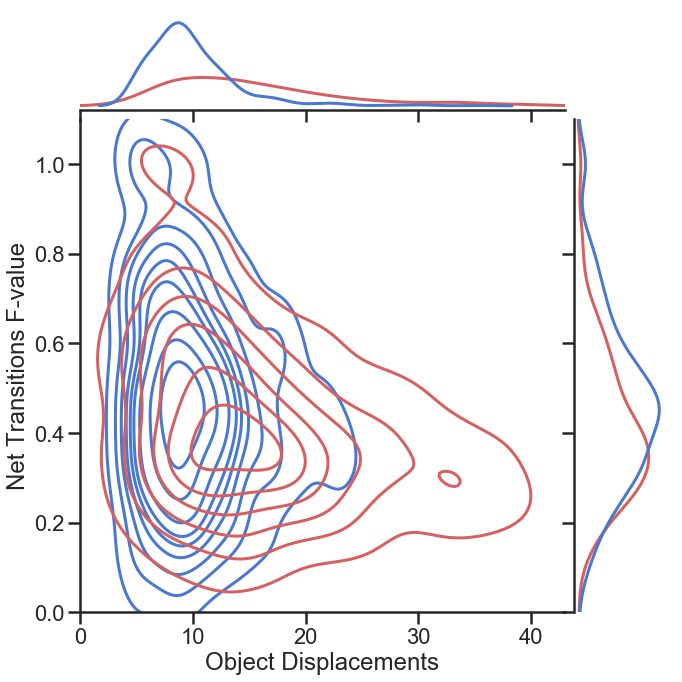
\includegraphics[width=0.3\linewidth]{source/figures/results/gaze_guidance_v_grasps_kde_execution.png}
    \label{figure:g_kde_exe}}
    \subfloat[]{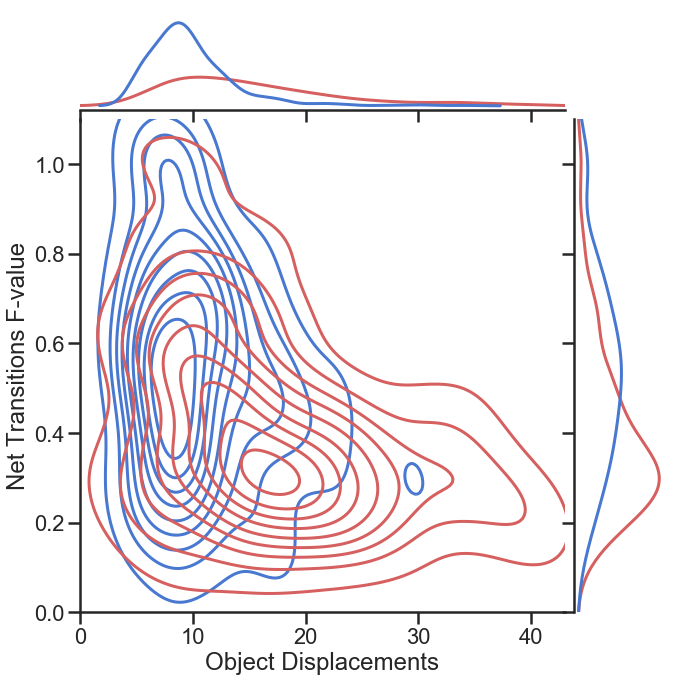
\includegraphics[width=0.3\linewidth]{source/figures/results/gaze_guidance_v_grasps_kde_planning.png}\label{figure:g_kde_plan}}
    \caption[]{Bi-variate kernel density estimate of net-transitions per trial vs. number of object displacement
    Panel \protect\subref{figure:g_kde_exe} shows kde of execution epochs
    Panel \protect\subref{figure:g_kde_plan} shows kde of planning epochs}
     \label{figure:kde}
\end{figure}

\begin{figure}[h]
    \centering
    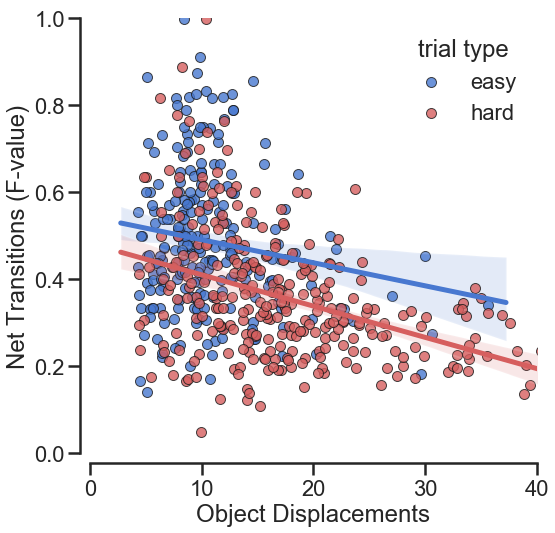
\includegraphics[width=0.3\linewidth]{source/figures/results/gaze_guidance_v_grasps_planning.png}
    \caption[]{Gaze guidance behavior vs. number of object displacements. Figure shows a scatter plot of the relative net transition (F-value) vs. number of object displacements per trial and subject differentiated the two trial types EASY(blue), HARD(red). Each point refers to one trial and it's F value vs. the number of object displacements in that trial. The lines denote the regression fit and the shaded region denotes 95\% confidence interval. F-values for both trial types decrease with increasing number of object displacements. Specifically, higher number of object displacements in a trial is correlated with lower gaze guidance. Pearson correlation $\rho$= -0.15 (p = 0.01) for EASY trials and $\rho$ = -0.38 (p <0.001) for HARD trials\\
    }
    \label{figure:F_value_plan}
\end{figure}